In order to use HJ-RA to solve a reachability problem in the case of a robot, we have to follow several steps. The first one is the definition of the game dynamics, that in the case of wheeled mobile robot, is usually given by its kinematic model where control input is the wheels velocities. The second step is the definition and computation of the Hamiltonian, in our case the definition is (\ref{h_m}) since we assume $u$ wants to minimize and $d$ to maximize. In addition to that, the numerical method \cite{new_paper} able to compute $V^+(x,t)$ requires also computation of its partial derivative w.r.t. the vector $p$. The third step is the environment definition, namely definition of $g(x,s)$ and $h(x,s)$ that represent respectively the reach set $\mathcal{R}_s$ and the constraint set $\mathcal{K}_s$ at the time $s$. The final step is the numerical computation of $V^+(x,t)$ using the algorithm in \cite{new_paper}, to do that we can use two Matlab libraries: ToolboxLS \cite{LS} and helperOC \cite{brief_intro}.

Once computed $V^+(x,t)$, in a limited and discretized state-time space, we can use this value function to define a safe control law from each feasible initial states $x_0$ to the reach set.

\subsection{Definition Game Dynamics}
Our case of study focuses on a three-wheeled omnidirectional mobile robot \cite{three_wheel} \cite{motion_control} which is a holonomic robot that has the ability to move simultaneously and independently in translation and rotation. The robot has three omni-wheels equally disposed at $120^\circ$, and have a distance $L$ from their center and the robot's center of mass $r \equiv O_m$.  

\begin{figure}[ht]
  \centering
  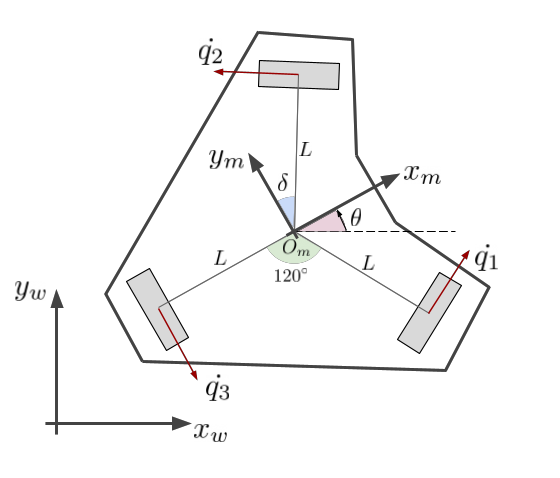
\includegraphics
      [width=0.35\textwidth]
      {figures/robot1.png}
  \caption{Three-wheeled omnidirectional mobile robot}
  \label{fig:robot_w}
\end{figure}

As shown in Fig. \ref{fig:robot_w}, there are two different reference frames: the first $RF_m \triangleq [O_m, X_m, Y_m]$ is a mobile frame placed at the robot's center of mass, the second one is the fixed world coordinate system $RF_w \triangleq [O_w, X_w, Y_w]$. Robot orientation w.r.t to $RF_w$ is given by the angle $\theta$. The angle $\delta$ is equal to $30^\circ$ and indicates the wheel orientation w.r.t. $RF_m$.

The kinematic model w.r.t. $RF_w$ is deduced as follows:

\begin{align}
    \dot{x} &= \begin{bmatrix}
           \frac{2}{3}\cos{(\theta + \delta)} & -\frac{2}{3}\cos{(\theta - \delta)} &  \frac{2}{3}\sin{\theta}   \\
           \frac{2}{3}\sin{(\theta + \delta)} & -\frac{2}{3}\sin{(\theta - \delta)} &  -\frac{2}{3}\cos{\theta} \\
           \frac{1}{3L} & \frac{1}{3L} & \frac{1}{3L}
         \end{bmatrix} \dot{q} 
  \label{eq:kin_model}
\end{align}
\begin{align*}
    &+ \begin{bmatrix}
         -sin{\theta} \\
         cos{\theta} \\
         0
        \end{bmatrix} d
\end{align*}

Where system state is given by $x = [^w x_r, ^w y_r, \theta]^T$, and the control input $u=[u_1, u_2, u_3]^T = \dot{q} = [\dot{q_1}, \dot{q_2}, \dot{q_3}]^T$ The second term represents an external disturbance given by a velocity with module $d$ and perpendicular to robot orientation $\theta$ (i.e. it lies on $Y_m$). We assume both inputs to be limited in an interval as required by game theory: $u \in U = [u_{min}, u_{max}]$, $d \in D = [d_{min}, d_{max}]$.
The procedure to calculate (\ref{eq:kin_model}) is shown in the Appendix.

\subsection{Hamiltonian}
The game dynamics $f(x(\cdot), u(\cdot), d(\cdot))$ is given by (\ref{eq:kin_model}), therefore the upper Hamiltonian can be computed as follows:
\begin{equation*}
  H^+(x,p,t) = \min_{u \in U}\max_{d \in D} [p_x, p_y, p_{\theta}]^T f(x, u, d)
\end{equation*}
Developing and collecting terms w.r.t. inputs \footnote{$c(\cdot)=\cos(\cdot)$, $s(\cdot)=\sin(\cdot)$}:
\begin{equation*}
  \begin{split}
    H^{+}(\cdot) = \min_{u \in U}\max_{d \in D} 
    &
      \begin{pmatrix}
        \frac{2}{3}c{(\theta + \delta)}p_x +  \frac{2}{3}s{(\theta + \delta }p_y + \frac{1}{3L}p_{\theta}
      \end{pmatrix}u_{1} 
    \\ +  
    &
      \begin{pmatrix}
        -\frac{2}{3}c{(\theta -\delta)}p_x -\frac{2}{3}s{(\theta -\delta)}p_y + \frac{1}{3L}p_{\theta} 
      \end{pmatrix}u_{2} 
    \\ +  
    &
      \begin{pmatrix}
        -\frac{2}{3}s{(\theta)}p_x -\frac{2}{3}c{(\theta)}p_y + \frac{1}{3L}p_{\theta} 
      \end{pmatrix}u_{3} 
    \\ + 
    &
      (c{(\theta)}p_y-s{(\theta)}p_x)d
  \end{split}
\end{equation*}
For the sake of brevity:
\begin{equation*}
  \begin{split}
    H^{+}(\cdot) = \min_{u \in U}\max_{d \in D} \sigma_{u1} u_{1} +\sigma_{u2} u_{2} + \sigma_{u3} u_{3} + \sigma_{d} d
  \end{split}
\end{equation*}

Since inputs appear linearly in the Hamiltonian, it is easy to solve the min-max problem, in other cases could be necessary to use optimization numerical tools:
\begin{equation}
  \begin{split}
    H^{+}(\cdot) = \sigma_{u1} u_{1}^* +\sigma_{u2} u_{2}^* + \sigma_{u3} u_{3}^* + \sigma_{d} d^*
  \end{split}
  \label{opt_ham}
\end{equation}
Where $u^* = [u_1^*, u_2^*, u_3^*]^T$ and $d^*$ represent the optimal moves for the two players and are given by:
\begin{equation}
  u_i = 
	\begin{cases} 
		u_{min} &\text{if } \sigma_{ui} \geq 0\\
		u_{max} &\text{Otherwise} 
	\end{cases}
\end{equation}

\begin{equation}
  d= 
	\begin{cases} 
		d_{min} &\text{if } \sigma_{d} \leq 0\\
		d_{max} &\text{Otherwise} 
	\end{cases}
  \label{opt_d}
\end{equation}
Please notice that these optimal inputs cannot be computed at prior since first they require the computation of $V^+(x,t)$ necessary to calculate $p = [p_x, p_y, p_{\theta}]^T$.

Finally, as required from the numerical method able to compute $V^+(x,t)$, we compute the partial derivative of (\ref{opt_ham}) w.r.t. to $p$. Please refer to \cite{new_paper} \cite{mitch_phd} for the mathematics reasons behind it.

\begin{equation}
  \frac{\partial H^+(x,p,t)}{\partial p} = 
    \left[
      \frac{\partial H^+(\cdot)}{\partial p_x},
      \frac{\partial H^+(\cdot)}{\partial p_y},
      \frac{\partial H^+(\cdot)}{\partial p_{\theta}}    
    \right]
\end{equation}
\begin{equation*}
  \begin{split}
    \frac{\partial H^+(x,p,t)}{\partial p_x} =
    &
    \frac{2}{3}cos(\theta+\delta)u_1^* - \frac{2}{3}cos(\theta-\delta)u_2^* \\
    &
    + \frac{2}{3}sin(\theta)u_3^* - sin(\theta)d^* \\
  \end{split}
\end{equation*}
\begin{equation*}
  \begin{split}
    \frac{\partial H^+(x,p,t)}{\partial p_y} =
    &
    \frac{2}{3}sin(\theta+\delta)u_1^* - \frac{2}{3}sin(\theta-\delta)u_2^* \\
    &
    - \frac{2}{3}cos(\theta)u_3^* + cos(\theta)d^* \\
  \end{split}
\end{equation*}
\begin{equation*}
    \frac{\partial H^+(x,p,t)}{\partial p_{\theta}} = \frac{u_1^* + u_2^* + u_3^*}{3L} 
\end{equation*}

We treat the final two steps of the case of study, namely environment definition and implementation, in the next section.



